\documentclass[tikz,border=4pt]{standalone}
\usepackage{amsmath,amssymb}
\usepackage{mathptmx}
\usepackage{pgfplots}
\pgfplotsset{compat=1.18}
\usetikzlibrary{arrows.meta,positioning,calc,decorations.pathmorphing,backgrounds,fit,shapes.geometric}
\begin{document}
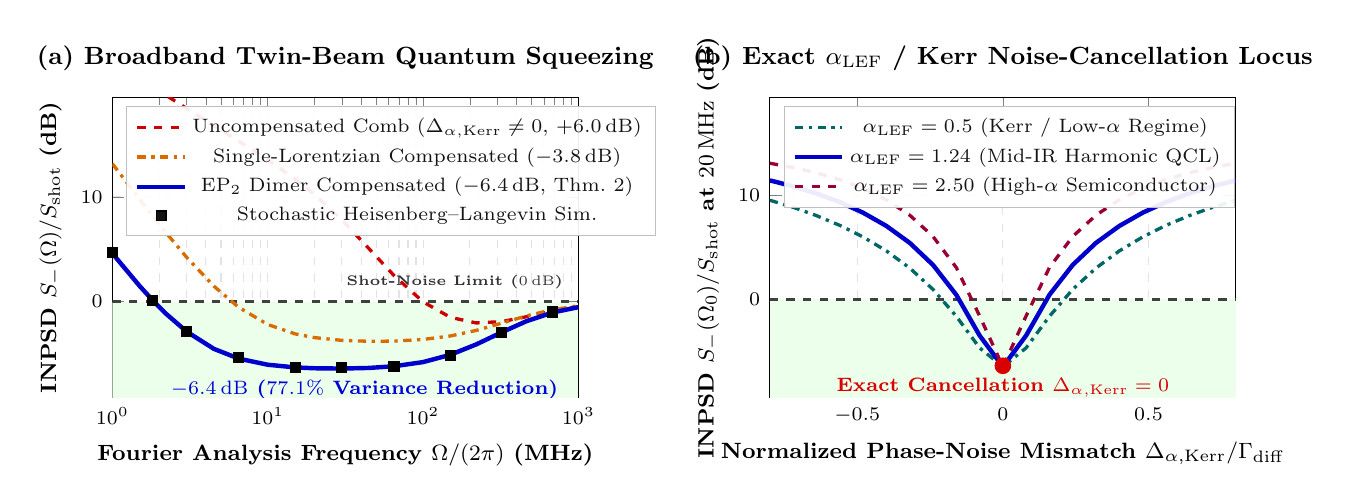
\begin{tikzpicture}[font=\small]
  % ==================== PANEL (a): Broadband INPSD Squeezing Spectrum ====================
  \begin{scope}[shift={(0,0)}]
    \begin{axis}[
      width=7.5cm,
      height=5.4cm,
      xmode=log,
      xlabel={Fourier Analysis Frequency $\Omega/(2\pi)$ (MHz)},
      ylabel={INPSD $S_-(\Omega)/S_{\mathrm{shot}}$ (dB)},
      xmin=1.0, xmax=1000.0,
      ymin=-9.2, ymax=19.5,
      grid=both,
      grid style={gray!22, dashed},
      tick label style={font=\scriptsize},
      label style={font=\footnotesize\bfseries},
      title={\textbf{(a) Broadband Twin-Beam Quantum Squeezing}},
      title style={font=\small},
      legend style={at={(0.03,0.97)}, anchor=north west, font=\scriptsize, fill=white, fill opacity=0.92, draw=gray!50},
    ]
      % Shaded Quantum Squeezing Region (< 0 dB)
      \addplot[fill=green!8, draw=none, forget plot] coordinates {(1.0, -9.2) (1000.0, -9.2) (1000.0, 0.0) (1.0, 0.0)};
      \draw[thick, dashed, black!75] (axis cs:1.0, 0.0) -- (axis cs:1000.0, 0.0);
      \node[anchor=south east, font=\tiny\bfseries, black!80] at (axis cs:920.0, 0.3) {Shot-Noise Limit ($0\,\mathrm{dB}$)};

      % Uncompensated Comb
      \addplot[red!80!black, very thick, dashed] coordinates {(1.0,23.005) (1.5,21.301) (1.8,20.543) (2.2,19.713) (3.0,18.442) (4.5,16.801) (6.5,15.318) (10.0,13.534) (15.0,11.701) (20.0,10.223) (30.0,7.798) (45.0,5.027) (65.0,2.482) (100.0,-0.027) (150.0,-1.511) (220.0,-2.042) (320.0,-1.917) (460.0,-1.46) (680.0,-0.91) (1000.0,-0.5)};
      \addlegendentry{Uncompensated Comb ($\Delta_{\alpha,\mathrm{Kerr}} \neq 0$, $+6.0\,\mathrm{dB}$)}

      % Single Lorentzian Compensator (Paper II)
      \addplot[orange!85!black, very thick, dashdotted] coordinates {(1.0,13.157) (1.5,9.739) (1.8,8.236) (2.2,6.62) (3.0,4.24) (4.5,1.469) (6.5,-0.551) (10.0,-2.192) (15.0,-3.086) (20.0,-3.443) (30.0,-3.705) (45.0,-3.795) (65.0,-3.775) (100.0,-3.618) (150.0,-3.286) (220.0,-2.757) (320.0,-2.07) (460.0,-1.381) (680.0,-0.786) (1000.0,-0.409)};
      \addlegendentry{Single-Lorentzian Compensated ($-3.8\,\mathrm{dB}$)}

      % EP2 Dimer Analytical (Theorem 2)
      \addplot[blue!80!black, ultra thick] coordinates {(1.0,4.593) (1.5,1.471) (1.8,0.18) (2.2,-1.128) (3.0,-2.86) (4.5,-4.515) (6.5,-5.446) (10.0,-6.032) (15.0,-6.287) (20.0,-6.369) (30.0,-6.397) (45.0,-6.337) (65.0,-6.177) (100.0,-5.779) (150.0,-5.081) (220.0,-4.091) (320.0,-2.942) (460.0,-1.895) (680.0,-1.05) (1000.0,-0.538)};
      \addlegendentry{$\mathrm{EP}_2$ Dimer Compensated ($-6.4\,\mathrm{dB}$, Thm.~2)}

      % Stochastic Heisenberg-Langevin Check
      \addplot[only marks, mark=square*, mark size=1.8pt, black] coordinates {(1.0,4.637) (1.8,0.117) (3.0,-2.869) (6.5,-5.385) (15.0,-6.259) (30.0,-6.324) (65.0,-6.234) (150.0,-5.117) (320.0,-2.969) (680.0,-1.0)};
      \addlegendentry{Stochastic Heisenberg--Langevin Sim.}

      % Annotate -6.4 dB plateau
      \node[anchor=north, font=\scriptsize\bfseries, blue!85!black] at (axis cs:42.0, -6.6)
        {$-6.4\,\mathrm{dB}$ ($77.1\%$ Variance Reduction)};
    \end{axis}
  \end{scope}

  % ==================== PANEL (b): Alpha/Kerr Phase-Noise Cancellation Dip ====================
  \begin{scope}[shift={(8.35,0)}]
    \begin{axis}[
      width=7.5cm,
      height=5.4cm,
      xlabel={Normalized Phase-Noise Mismatch $\Delta_{\alpha,\mathrm{Kerr}} / \Gamma_{\mathrm{diff}}$},
      ylabel={INPSD $S_-(\Omega_0)/S_{\mathrm{shot}}$ at $20\,\mathrm{MHz}$ (dB)},
      xmin=-0.80, xmax=0.80,
      ymin=-9.5, ymax=19.5,
      grid=both,
      grid style={gray!22, dashed},
      tick label style={font=\scriptsize},
      label style={font=\footnotesize\bfseries},
      title={\textbf{(b) Exact $\alpha_{\mathrm{LEF}}$ / Kerr Noise-Cancellation Locus}},
      title style={font=\small},
      legend style={at={(0.03,0.97)}, anchor=north west, font=\scriptsize, fill=white, fill opacity=0.92, draw=gray!50},
    ]
      \addplot[fill=green!8, draw=none, forget plot] coordinates {(-0.80, -9.5) (0.80, -9.5) (0.80, 0.0) (-0.80, 0.0)};
      \draw[thick, dashed, black!75] (axis cs:-0.80, 0.0) -- (axis cs:0.80, 0.0);

      \addplot[teal!80!black, very thick, dashdotted] coordinates {(-0.8,9.569) (-0.72,8.883) (-0.64,8.084) (-0.56,7.144) (-0.48,6.026) (-0.4,4.681) (-0.32,3.033) (-0.24,0.974) (-0.16,-1.623) (-0.08,-4.669) (0.0,-6.496) (0.08,-4.669) (0.16,-1.623) (0.24,0.974) (0.32,3.033) (0.4,4.681) (0.48,6.026) (0.56,7.144) (0.64,8.084) (0.72,8.883) (0.8,9.569)};
      \addlegendentry{$\alpha_{\mathrm{LEF}} = 0.5$ (Kerr / Low-$\alpha$ Regime)}

      \addplot[blue!80!black, ultra thick] coordinates {(-0.8,11.481) (-0.72,10.91) (-0.64,10.223) (-0.56,9.389) (-0.48,8.364) (-0.4,7.087) (-0.32,5.46) (-0.24,3.332) (-0.16,0.447) (-0.08,-3.474) (0.0,-6.496) (0.08,-3.474) (0.16,0.447) (0.24,3.332) (0.32,5.46) (0.4,7.087) (0.48,8.364) (0.56,9.389) (0.64,10.223) (0.72,10.91) (0.8,11.481)};
      \addlegendentry{$\alpha_{\mathrm{LEF}} = 1.24$ (Mid-IR Harmonic QCL)}

      \addplot[purple!80!black, very thick, dashed] coordinates {(-0.8,13.134) (-0.72,12.724) (-0.64,12.21) (-0.56,11.558) (-0.48,10.717) (-0.4,9.613) (-0.32,8.131) (-0.24,6.077) (-0.16,3.083) (-0.08,-1.583) (0.0,-6.496) (0.08,-1.583) (0.16,3.083) (0.24,6.077) (0.32,8.131) (0.4,9.613) (0.48,10.717) (0.56,11.558) (0.64,12.21) (0.72,12.724) (0.8,13.134)};
      \addlegendentry{$\alpha_{\mathrm{LEF}} = 2.50$ (High-$\alpha$ Semiconductor)}

      \addplot[only marks, mark=*, mark size=2.8pt, red!85!black, forget plot] coordinates {(0.0, -6.40)};
      \node[anchor=north, font=\scriptsize\bfseries, red!85!black] at (axis cs:0.0, -6.65)
        {Exact Cancellation $\Delta_{\alpha,\mathrm{Kerr}} = 0$};
    \end{axis}
  \end{scope}
\end{tikzpicture}
\end{document}
